% Options for packages loaded elsewhere
\PassOptionsToPackage{unicode}{hyperref}
\PassOptionsToPackage{hyphens}{url}
%
\documentclass[
]{article}
\usepackage{amsmath,amssymb}
\usepackage{lmodern}
\usepackage{iftex}
\ifPDFTeX
  \usepackage[T1]{fontenc}
  \usepackage[utf8]{inputenc}
  \usepackage{textcomp} % provide euro and other symbols
\else % if luatex or xetex
  \usepackage{unicode-math}
  \defaultfontfeatures{Scale=MatchLowercase}
  \defaultfontfeatures[\rmfamily]{Ligatures=TeX,Scale=1}
\fi
% Use upquote if available, for straight quotes in verbatim environments
\IfFileExists{upquote.sty}{\usepackage{upquote}}{}
\IfFileExists{microtype.sty}{% use microtype if available
  \usepackage[]{microtype}
  \UseMicrotypeSet[protrusion]{basicmath} % disable protrusion for tt fonts
}{}
\makeatletter
\@ifundefined{KOMAClassName}{% if non-KOMA class
  \IfFileExists{parskip.sty}{%
    \usepackage{parskip}
  }{% else
    \setlength{\parindent}{0pt}
    \setlength{\parskip}{6pt plus 2pt minus 1pt}}
}{% if KOMA class
  \KOMAoptions{parskip=half}}
\makeatother
\usepackage{xcolor}
\usepackage[margin=1in]{geometry}
\usepackage{color}
\usepackage{fancyvrb}
\newcommand{\VerbBar}{|}
\newcommand{\VERB}{\Verb[commandchars=\\\{\}]}
\DefineVerbatimEnvironment{Highlighting}{Verbatim}{commandchars=\\\{\}}
% Add ',fontsize=\small' for more characters per line
\usepackage{framed}
\definecolor{shadecolor}{RGB}{248,248,248}
\newenvironment{Shaded}{\begin{snugshade}}{\end{snugshade}}
\newcommand{\AlertTok}[1]{\textcolor[rgb]{0.94,0.16,0.16}{#1}}
\newcommand{\AnnotationTok}[1]{\textcolor[rgb]{0.56,0.35,0.01}{\textbf{\textit{#1}}}}
\newcommand{\AttributeTok}[1]{\textcolor[rgb]{0.77,0.63,0.00}{#1}}
\newcommand{\BaseNTok}[1]{\textcolor[rgb]{0.00,0.00,0.81}{#1}}
\newcommand{\BuiltInTok}[1]{#1}
\newcommand{\CharTok}[1]{\textcolor[rgb]{0.31,0.60,0.02}{#1}}
\newcommand{\CommentTok}[1]{\textcolor[rgb]{0.56,0.35,0.01}{\textit{#1}}}
\newcommand{\CommentVarTok}[1]{\textcolor[rgb]{0.56,0.35,0.01}{\textbf{\textit{#1}}}}
\newcommand{\ConstantTok}[1]{\textcolor[rgb]{0.00,0.00,0.00}{#1}}
\newcommand{\ControlFlowTok}[1]{\textcolor[rgb]{0.13,0.29,0.53}{\textbf{#1}}}
\newcommand{\DataTypeTok}[1]{\textcolor[rgb]{0.13,0.29,0.53}{#1}}
\newcommand{\DecValTok}[1]{\textcolor[rgb]{0.00,0.00,0.81}{#1}}
\newcommand{\DocumentationTok}[1]{\textcolor[rgb]{0.56,0.35,0.01}{\textbf{\textit{#1}}}}
\newcommand{\ErrorTok}[1]{\textcolor[rgb]{0.64,0.00,0.00}{\textbf{#1}}}
\newcommand{\ExtensionTok}[1]{#1}
\newcommand{\FloatTok}[1]{\textcolor[rgb]{0.00,0.00,0.81}{#1}}
\newcommand{\FunctionTok}[1]{\textcolor[rgb]{0.00,0.00,0.00}{#1}}
\newcommand{\ImportTok}[1]{#1}
\newcommand{\InformationTok}[1]{\textcolor[rgb]{0.56,0.35,0.01}{\textbf{\textit{#1}}}}
\newcommand{\KeywordTok}[1]{\textcolor[rgb]{0.13,0.29,0.53}{\textbf{#1}}}
\newcommand{\NormalTok}[1]{#1}
\newcommand{\OperatorTok}[1]{\textcolor[rgb]{0.81,0.36,0.00}{\textbf{#1}}}
\newcommand{\OtherTok}[1]{\textcolor[rgb]{0.56,0.35,0.01}{#1}}
\newcommand{\PreprocessorTok}[1]{\textcolor[rgb]{0.56,0.35,0.01}{\textit{#1}}}
\newcommand{\RegionMarkerTok}[1]{#1}
\newcommand{\SpecialCharTok}[1]{\textcolor[rgb]{0.00,0.00,0.00}{#1}}
\newcommand{\SpecialStringTok}[1]{\textcolor[rgb]{0.31,0.60,0.02}{#1}}
\newcommand{\StringTok}[1]{\textcolor[rgb]{0.31,0.60,0.02}{#1}}
\newcommand{\VariableTok}[1]{\textcolor[rgb]{0.00,0.00,0.00}{#1}}
\newcommand{\VerbatimStringTok}[1]{\textcolor[rgb]{0.31,0.60,0.02}{#1}}
\newcommand{\WarningTok}[1]{\textcolor[rgb]{0.56,0.35,0.01}{\textbf{\textit{#1}}}}
\usepackage{graphicx}
\makeatletter
\def\maxwidth{\ifdim\Gin@nat@width>\linewidth\linewidth\else\Gin@nat@width\fi}
\def\maxheight{\ifdim\Gin@nat@height>\textheight\textheight\else\Gin@nat@height\fi}
\makeatother
% Scale images if necessary, so that they will not overflow the page
% margins by default, and it is still possible to overwrite the defaults
% using explicit options in \includegraphics[width, height, ...]{}
\setkeys{Gin}{width=\maxwidth,height=\maxheight,keepaspectratio}
% Set default figure placement to htbp
\makeatletter
\def\fps@figure{htbp}
\makeatother
\setlength{\emergencystretch}{3em} % prevent overfull lines
\providecommand{\tightlist}{%
  \setlength{\itemsep}{0pt}\setlength{\parskip}{0pt}}
\setcounter{secnumdepth}{-\maxdimen} % remove section numbering
\ifLuaTeX
  \usepackage{selnolig}  % disable illegal ligatures
\fi
\IfFileExists{bookmark.sty}{\usepackage{bookmark}}{\usepackage{hyperref}}
\IfFileExists{xurl.sty}{\usepackage{xurl}}{} % add URL line breaks if available
\urlstyle{same} % disable monospaced font for URLs
\hypersetup{
  pdftitle={london.etal.manuscript.appendix},
  hidelinks,
  pdfcreator={LaTeX via pandoc}}

\title{london.etal.manuscript.appendix}
\author{}
\date{\vspace{-2.5em}2022-07-15}

\begin{document}
\maketitle

\hypertarget{supplementary-material}{%
\section{Supplementary Material}\label{supplementary-material}}

\hypertarget{methods}{%
\subsection{Methods}\label{methods}}

\hypertarget{subjects}{%
\subsubsection{Subjects}\label{subjects}}

Our study population of 20 Pinyon Jays (\emph{Gymnorhinus
cyanocephalus}) were wild born and locally housed. Researchers captured
these birds in either Arizona or California (United States Fish and
Wildlife permit MB694205) between 2006 and 2011. At capture, they were
estimated to be between one and three years of age. The colony has an
age range of 12, 17 years with a mean of 14.4516129years . The
University of Nebraska-Lincoln Institutional Animal Care and Use
Committee approved this project (protocol number 1867 and 2059), and all
procedures conformed to the ASAB/ABS Guidelines for the use of animals
in research. All subjects have completed prior cognitive and behavioral
experiments in their tenure with the lab. The colony is handled by
humans extensively.

Repetition 1: Eight Pinyon Jays (one female) completed all rounds of the
food experiment and 10 Pinyon Jays (four female) completed all rounds of
the social experiment. The Pinyon Jays in the food item experiment were
housed two to a double cage, while the jays in the social experiment
were individually housed. A further 17 Pinyon Jays (six female) from the
colony were used as stooge conspecifics in the social experiment. This
number includes six birds that had to be transferred out of use as
stooge birds due to unrelated colony matters. Stooge birds were
primarily housed socially and always in a separate room from the testing
subjects. Two Pinyon Jays were dropped from the social experiment due to
unrelated health concerns.

Repetition 2: Four Pinyon Jays (\# female) completed all rounds of the
food experiment and Ten Pinyon Jays (\# female) completed all rounds of
the social experiment. A further 8 Pinyon Jays (\# female) from the
colony were used as stooge conspecifics in the social experiment.
Housing was the same in both repetitions.

\hypertarget{food-item-habituation-and-training}{%
\subsubsection{Food Item Habituation and
Training}\label{food-item-habituation-and-training}}

Prior to experimental sessions, all birds had to be habituated to the
experimental room, cage, and stand and then experience training.
Depending on the bird this took between 9-16 weeks as each bird was ran
once a day between 11:00-13:00 CST. Subjects experienced four training
phases in total; each aimed at teaching the bird a different piece of
the paradigm. The first phase (rear cup habituation) habituated subjects
to the apparatus. The second phase (front dish habituation) encouraged
the birds to place their heads through holes at the front of the cage to
consume mealworms from the dishes on the trays. The third phase (moving
dish training) introduced the subjects to the fact that the dish on the
unchosen side moved out of reach. The forth phase (mixed reward
training) taught the subjects to quickly make a choice between zero or
three mealworms, eat, and then set up for another trial in quick
succession.

For rear cup habituation, the experimenter brought a subject from their
home cage and released them into the test cage. Five mealworms were
placed in each of the two feeding bowls into slots at the back of the
cage. After three minutes, the experimenter counted the number of
mealworms consumed in each food dish and returned the subject to its
home cage.

For front dish habituation, the experimenter brought a subject from
their home cage into the test cage. Three mealworms were placed in both
dishes on the Plexiglass trays. The experimenter pushed the trays
forward to present the dishes to the subject in one swift and smooth
motion. After three minutes, the experimenter counted the number of
mealworms eaten in each dish and returned the subject to their home
cage.

Moving dish training was identical to front dish habituation, except the
experimenter pulled back the tray in front of the unchosen perch. If
subjects ate all three mealworms before three minutes expired, we
repeated this process. If the bird did not finish their mealworms we
waited the rest of the three minutes before returning them to their home
cage.

The mixed reward training was identical to the moving dish training,
except one of the dishes held no mealworms while the other held three
mealworms and subjects completed six of these 30 second trials per
session.

Subjects progressed to a new phase when they successfully consumed at
least 70\% of the mealworms offered in their current phase for three
consecutive days. Subjects could also move to a previous phase if they
consumed less than 25\% of the mealworms offered on five out of seven
days of training.

\hypertarget{food-experimental-procedure}{%
\subsubsection{Food Experimental
Procedure}\label{food-experimental-procedure}}

All experimental sessions ran between 11:00-13:00 CST to keep the birds'
hunger levels constant throughout the experiment. The subjects were not
food restricted and were fed three hours prior to the start of the
experiment. One experimenter conducted each session. The first trial of
the session consisted of one round of mixed reward training. If they
failed this check, the experimenter completed two more rounds of mixed
reward training. If they failed two out of three of these trials this
triggers de-bias training. If they succeed, they continued to the
experimental trials. For these trials, the experimenter placed the
appropriate number of mealworms in each of the dishes, with mealworms
placed 2.5 cm away from each other. The subject then started the trial
on the back perch and hopped forward to one of the front perches to
signal choice. The experimenter then removed the opposite dish and the
subject had up to three minutes to consume their mealworms. If the
subject did not make a choice and/or finish all mealworms within 3
minutes, we ended the session. Once the subject consumed all mealworms,
we immediately started the next trial. The first trial of the day where
the subject did not finish all their chosen mealworms triggered a stop
on that days session. Subjects completed on average 4 trials per
session.

Each bird experienced 10 repetitions for each of the 15 numerical pairs
between 1 and 6 (e.g., 6 vs 5, 6 vs 4, 6 vs 3, etc.). The side of the
larger option was pseudo randomized with no left or right runs longer
than three in a row. We organized the pairs into 10 blocks. Each block
was randomized within itself and had one instance of each factorial
pair. The order the subjects ran in a particular day was also
randomized.

\hypertarget{food-side-bias-protocol}{%
\subsubsection{Food Side-Bias Protocol}\label{food-side-bias-protocol}}

During habituation, three consecutive days of no choices and/or no
eating of mealworms on one particular side triggered side de-bias
training. During experimental sessions, there were two triggers for
de-bias training: either not completing the first 0 vs.~3 practice test
trial correctly or when a bird chose the same side for 10 consecutive
trials. De-biasing training consisted of three mealworms placed in the
dish the subject avoided and no mealworms in the side they preferred.
The subject was allowed up to one minute to select the dish that
contained mealworms. If the bird did not make a choice or eat any
mealworms in the allotted time, we slide both trays all the way out of
the stand, placed them out of view of the bird, waited a few seconds,
then began the trial over. If they ate within the minute, we reset as
soon as they ate until they had five total opportunities to eat. The
bird returned to habituation or experimental sessions once they
successfully chose the avoided side immediately and ate at least 60\% of
the mealworms provided.

\hypertarget{food-apparatus}{%
\subsubsection{Food Apparatus}\label{food-apparatus}}

The apparatus for the food experiment included a bird cage (72 x 48 x 48
cm) abutting a plastic stand with sliding trays that contained mealworms
(Figure \ref{fig:foodapp}). The stand was set at a 15 degree angle
tilted toward the subject to facilitate mealworm viewing. The stand had
two pvc pipe lined channels the same width as our plexiglass trays. Each
plexiglass tray had a standard petri dish placed half an inch away from
the front of each tray. Mealworms were placed in the front two thirds of
the petri dish so the subjects could easily reach the mealworms and they
were evenly distributed across the available area. Within the cage were
three perches. One large free standing perch stood in the middle of the
cage, while two small perches attached to each side of the cage a few
inches back from the front. Subjects started each trial perched on the
large free standing perch, and they chose an option by landing on the
smaller left or right perches. They then consumed the mealworms
associated with their decision while the unchosen side was removed
immediately.

(ref:foodapp-cap) Food experiment apparatus (overhead view).

\begin{Shaded}
\begin{Highlighting}[]
\FunctionTok{include\_graphics}\NormalTok{(}\FunctionTok{here}\NormalTok{(}\StringTok{"figures/food\_apparatus.PNG"}\NormalTok{))}
\end{Highlighting}
\end{Shaded}

\begin{figure}

{\centering 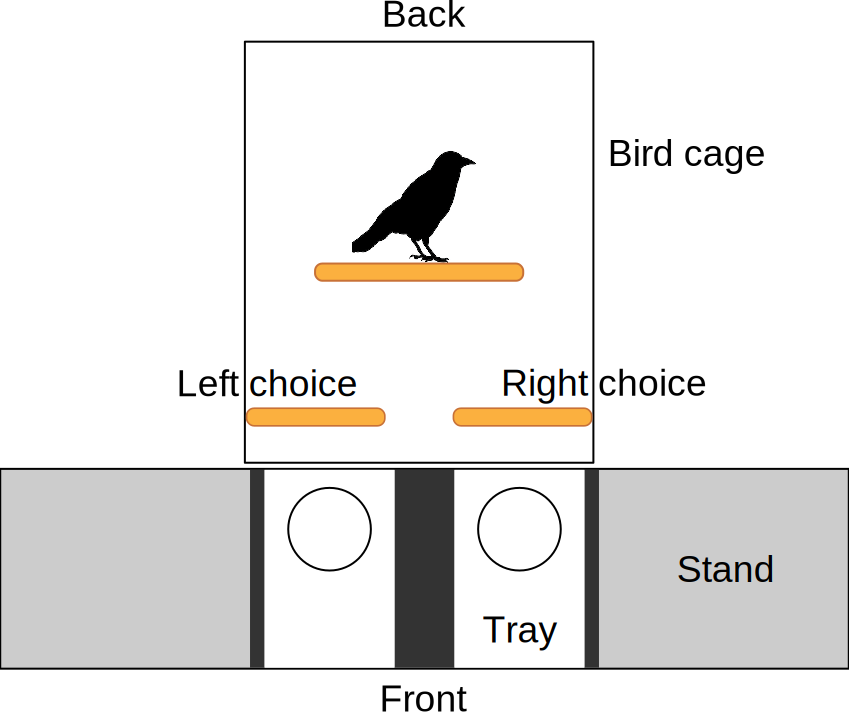
\includegraphics[width=1\linewidth]{../figures/food_apparatus} 

}

\caption{(ref:socialapp-cap)}\label{fig:foodapp}
\end{figure}

\hypertarget{social-experiment-habitutation-and-training}{%
\subsubsection{Social Experiment habitutation and
Training}\label{social-experiment-habitutation-and-training}}

Prior to experimentation, we habituated all birds to both the
experimental room and the apparatus. For habituation, we attached a
stainless steal cup to the front of each bird cage. For a habituation
session, the experimenter placed five mealworms in each of the cups. The
experimenter then brought the subject into the room, pulled up both
doors, and showed the subject each arm of the maze for six seconds,
randomizing between subjects the side shown first. The subject was then
gently placed on the bottom of the testing chamber as close to the
center as possible with the bird facing away from their options. Once
the subject crossed the threshold of a door, the door was quietly and
swiftly closed behind them and the bird explored the chosen arm and
consumed the mealworms for two minutes. After the two minutes expired,
the experimenter removed the subject from the apparatus and recorded the
number of mealworms consumed.

Subjects experienced 1 habituation session per day for 5 days a week.
They completed habituation once they consistently consumed at least 80\%
of the mealworms offered to them in both arms of the apparatus and had
no significant signs of a side bias. Depending on the bird, this took
between 4-6 weeks.

\hypertarget{social-experimental-procedure}{%
\subsubsection{Social Experimental
Procedure}\label{social-experimental-procedure}}

All experimental trials ran between 09:00-11:00 CST. The subjects were
not food restricted. Two experimenters were present at each session: the
`handler' handled the subject, while the `recorder' handled the camera,
whiteboard, and the guillotine doors. The experimenter placed stooge
birds in their respective cages and allowed them to acclimate to the
room for 10 minutes before experimentation. The handler then placed the
subject inside the apparatus and showed them each option for six seconds
(counter balancing which was shown first) before releasing the subject
into the chamber. Once the subject crossed the threshold of one of the
doors, the recorder closed \emph{both} doors gently but swiftly. After
three minutes elapsed, the handler collected the subject and returned
them to their home cage. These steps repeated until all birds had run
through the experiment.

Repetition 1: Each subject experienced 5 repetitions for each of the 21
numerical pairs between 0 and 6 (e.g., 6 vs 5, 6 vs 4, 6 vs 3, etc.).
The side of the larger option was pseudo randomized with no left or
right runs longer than 3 in a row. The pairs were organized into blocks
with one instance of each pair per block and pairs randomized within
each block. The order in which the subjects ran in a particular day was
also randomized. Only the 15 numerical pairs between 1 and 6 were
analyzed.

Repetition 2: Each bird experienced 10 repetitions for each of the 15
numerical pairs between 1 and 6 (e.g., 6 vs 5, 6 vs 4, 6 vs 3, etc.).
Randomization was the same for both repetitions.

\hypertarget{social-side-bias-protocol}{%
\subsubsection{Social Side-Bias
Protocol}\label{social-side-bias-protocol}}

If any subject chose either the left or right side for six consecutive
sessions in either habituation or experimentation, they experienced side
de-biasing. For side de-biasing, only one door was open in the
apparatus, the door leading to the side the subject avoided. We placed
five mealworms in the food cup at the end of that arm with no stooge
birds present. The bird had up to five minutes to walk/fly past the door
into the correct side and three minutes once the door shut behind them
to eat the mealworms. Subjects experienced five consecutive trials in a
de-biasing session. The subject returned to habituation or experimental
sessions once they successfully choose the avoided side immediately upon
release and ate at least 60\% of the mealworms provided.

\hypertarget{social-apparatus}{%
\subsubsection{Social Apparatus}\label{social-apparatus}}

The apparatus (Figure \ref{fig:socialapp}) took the form of a Y maze
formed out of chicken wire, plastic sheets, and Plexiglas. The subject
entered a large chamber at the base of the maze before choosing one of
two arms of the Y maze. At the entrance to both arms, a guillotine style
door was closed after the bird walked or flew past it, thus making a
choice between the option on the left or right. At the end of each arm,
was a large bird cage housing the stooge birds. Each cage had two
lengthwise perches for the stooge birds to use and one small perch
hanging from the ceiling.

(ref:socialapp-cap) Social experiment apparatus (overhead view).

\begin{Shaded}
\begin{Highlighting}[]
\FunctionTok{include\_graphics}\NormalTok{(}\FunctionTok{here}\NormalTok{(}\StringTok{"figures/social\_apparatus.PNG"}\NormalTok{))}
\end{Highlighting}
\end{Shaded}

\begin{figure}

{\centering 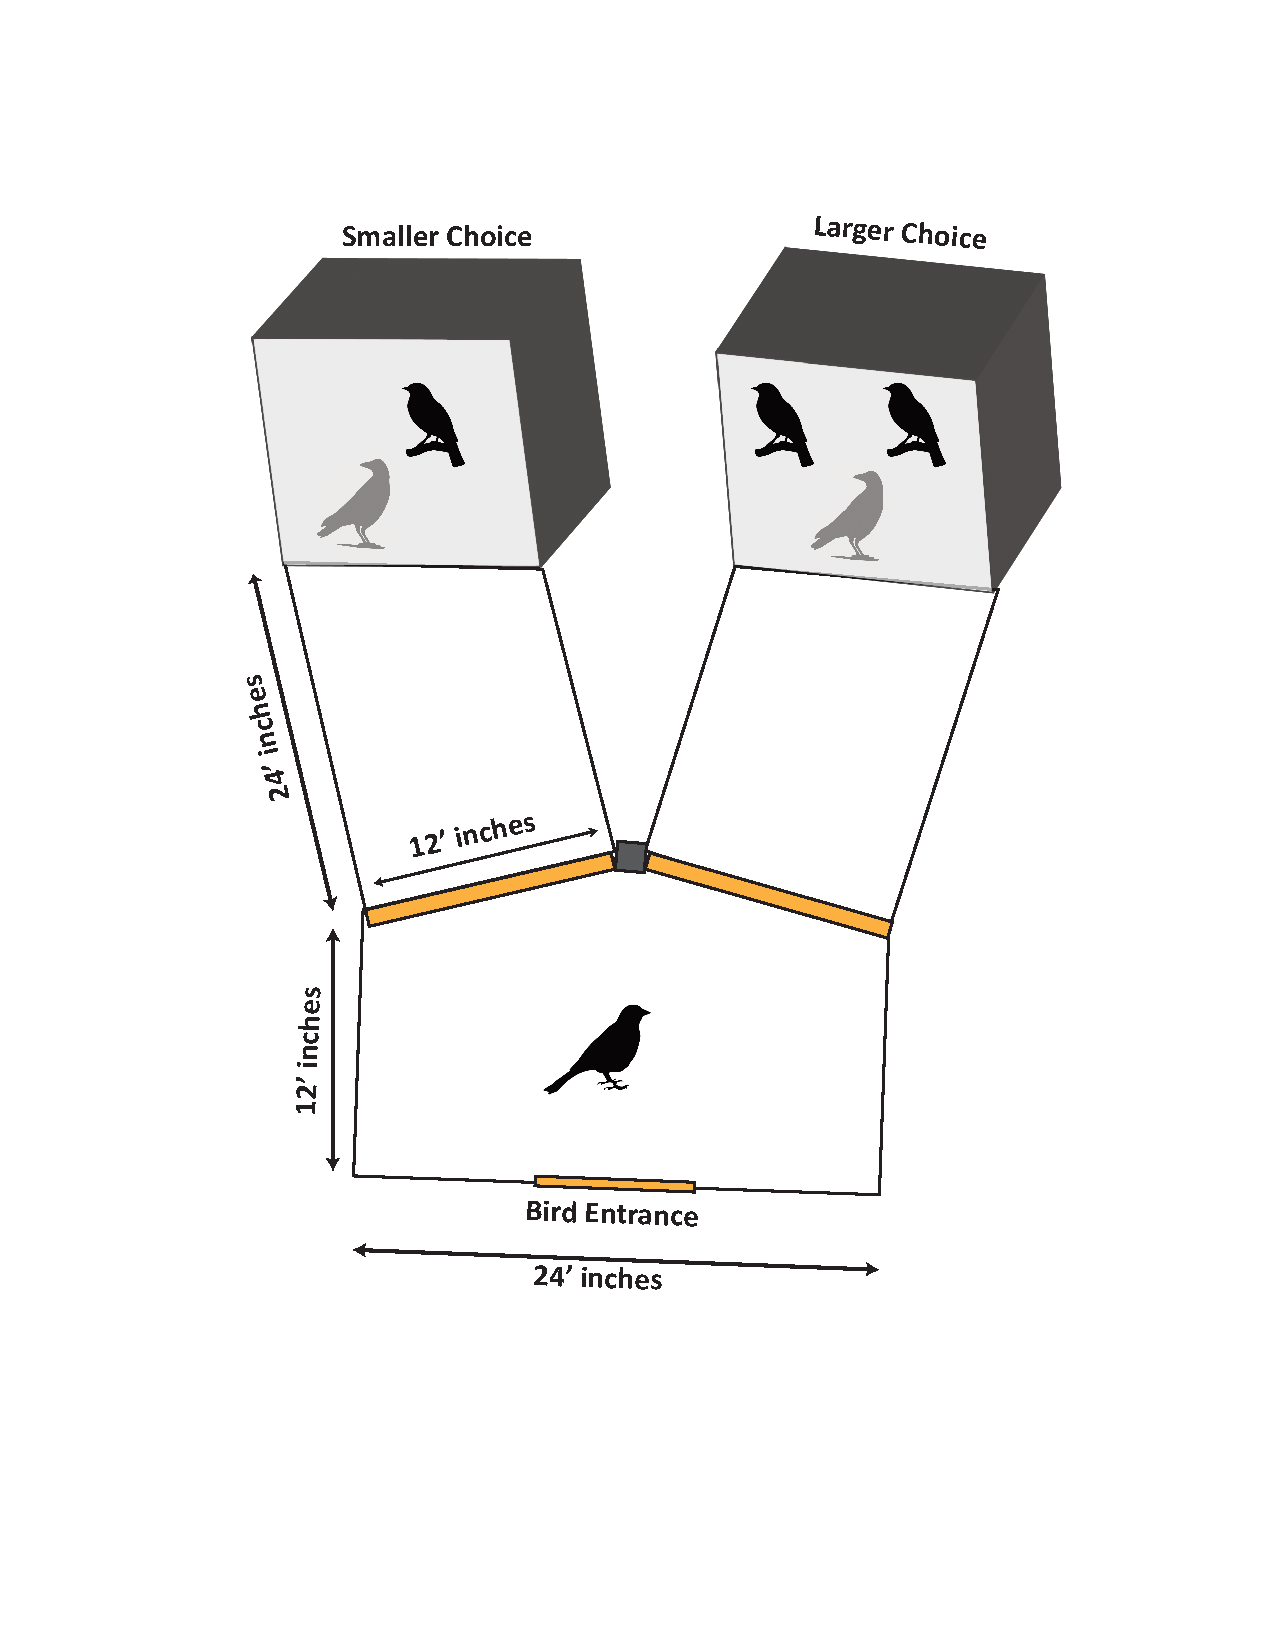
\includegraphics[width=1\linewidth]{../figures/social_apparatus} 

}

\caption{(ref:socialapp-cap)}\label{fig:socialapp}
\end{figure}

\#Data Analysis Data were analyzed and processed for the project using R
{[}Version 4.2.1\textbackslash; @R-base{]} and the R-packages
\emph{BayesFactor} {[}Version 0.9.12.4.4\textbackslash;
@R-BayesFactor{]}, \emph{bayestestR} {[}Version 0.12.1\textbackslash;
@R-bayestestR{]}, \emph{BMA} {[}@R-BMA{]}, \emph{broom} {[}Version
1.0.0\textbackslash; @R-broom{]}, \emph{coda} {[}Version
0.19.4\textbackslash; @R-coda{]}, \emph{dplyr} {[}Version
1.0.9\textbackslash; @R-dplyr{]}, \emph{forcats} {[}Version
0.5.1\textbackslash; @R-forcats{]}, \emph{formattable} {[}Version
0.2.1\textbackslash; @R-formattable{]}, \emph{ggplot2} {[}Version
3.3.6\textbackslash; @R-ggplot2{]}, \emph{here} {[}Version
1.0.1\textbackslash; @R-here{]}, \emph{inline} {[}@R-inline{]},
\emph{knitr} {[}Version 1.39\textbackslash; @R-knitr{]}, \emph{leaps}
{[}@R-leaps{]}, \emph{lme4} {[}Version 1.1.30\textbackslash; @R-lme4{]},
\emph{Matrix} {[}Version 1.4.1\textbackslash; @R-Matrix{]},
\emph{papaja} {[}Version 0.1.1\textbackslash; @R-papaja{]},
\emph{patchwork} {[}Version 1.1.1\textbackslash; @R-patchwork{]},
\emph{performance} {[}Version 0.9.1\textbackslash; @R-performance{]},
\emph{purrr} {[}Version 0.3.4\textbackslash; @R-purrr{]}, \emph{readr}
{[}Version 2.1.2\textbackslash; @R-readr{]}, \emph{readxl} {[}Version
1.4.0\textbackslash; @R-readxl{]}, \emph{robustbase} {[}Version
0.95.0\textbackslash; @R-robustbase{]}, \emph{rrcov} {[}@R-rrcov{]},
\emph{stringr} {[}Version 1.4.0\textbackslash; @R-stringr{]},
\emph{survival} {[}Version 3.3.1\textbackslash; @R-survival-book{]},
\emph{tibble} {[}Version 3.1.8\textbackslash; @R-tibble{]}, \emph{tidyr}
{[}Version 1.2.0\textbackslash; @R-tidyr{]}, \emph{tidyverse} {[}Version
1.3.2\textbackslash; @R-tidyverse{]}, and \emph{tinylabels} {[}Version
0.2.3\textbackslash; @R-tinylabels{]}.

Prior to analysis, we transformed the left and right choice variable
from each trial into a binary operator, with 1 representing a choice for
the larger option and 0 representing a choice for the smaller option. We
also created variables with the numerical difference between each number
pair by subtracting the larger number from the smaller (6-1 = 5), as
well as creating the ratio by dividing the smaller by the larger number
(1/6 = 0.16). Our hypotheses explore the relationship between our binary
outcome variable, choice of the larger or smaller stimuli, and which
possible mechanism, difference or ratio, subjects use to make choices
when presented with either food or social items.

Our first hypothesis investigated whether pinyon jays prefer larger over
smaller numbers of food items and conspecifics. To test this, we
conducted a one sample t-tests of preference for larger numbers.
Therefore, we calculated the mean \emph{percent preference for larger
numbers} for each subject and used the t-test to compare the subject
means to 50. We perform both frequentist and Bayesian t-tests, with
inferences based on Bayes factors. Bayes factors for t-tests were
calculated using the \texttt{ttestBF} function from the
\emph{BayesFactor} R package {[}@Morey.etal.2021{]} using default,
noninformative priors.

Our second hypothesis investigated whether numerical difference and
ratio predict preferences between smaller and larger options and the
third hypothesis investigated whether difference and ratio predicted
preferences \emph{independently}. To test these hypotheses, we used
generalized linear mixed-effects modeling because the response variable
was dichotomous and our subjects repeatedly made decision on the same
number pairs. We used the trial-level choices for either the larger
(coded as 1) or smaller (coded as 0) option available in the number pair
as the response variable. To investigate our hypotheses, we used
generalized logistic models to compare which combination of random
(subject, pair, or both) and fixed (ratio, difference, or a combination
of both) effects best describe each data set (food and social). We first
found the best-fitting random effect structure, then added this random
structure to all of the possible fixed effect structures, leaving us
with the final best fitting model for each data set overall.

To explore random effect structure, we included models with no fixed
effect and either (1) no random effects (intercept only), (2) subject as
a random effect, (3) number pair as a random effect (to account for each
bird repeatedly seeing each pair multiple times), and (4) both subject
and number pair as random effects. For example, the model with both
subject and pair as random effects ran using the \texttt{glmer()}
function with the following structure:
\texttt{r\ glmer(choice\ \textasciitilde{}\ (1\textbar{}subject)+\ (1\textbar{}pair),\ family\ =\ binomial)}
(Figure \emph{A1} a). We then used Bayes factors to select the model
with the best-fitting random effect structure. We added the chosen
random effect structure to our fixed effects to find the best-fitting
model for the data set overall. The five fixed effects models were: (1)
no fixed effects (intercept only), (2) ratio as a fixed effect, (3)
difference as a fixed effect, (4) both difference and ratio as a fixed
effects but \emph{without} an interaction, and (5) both difference and
ratio as fixed effects \emph{with} an interaction. The model with both
difference and ratio as fixed effects with an interaction term ran using
the \texttt{glm()} function and the following structure:
\texttt{r\ glm(choice\ \textasciitilde{}\ difference\ *\ ratio,\ family\ =\ binomial)}
(Figure \emph{A1} b). We calculated Bayes factors using the
\texttt{test\_performance()} function from the \emph{performance}
package {[}@Ludeckestrengejacke.etal.2021{]}, which estimates Bayes
factors from model BIC values using Wagenmakers' {[}@Wagenmakers.2007{]}
equation. The best fitting model has the highest Bayes factor. The
second hypothesis will be supported if difference and ratio are both
included as main effects in the best fitting model. The third hypothesis
will be supported if the interaction between difference and ratio is
included in the best fitting model.

\renewcommand{\thetable}{A\arabic{table}}
\setcounter{table}{0}
\renewcommand{\thefigure}{A\arabic{figure}}

\setcounter{figure}{0}

(ref:pairstable-cap) Factorial pair combinations used each experiment.
We used every factorial pair from 1 to 6 resulting in 15 combinations.
The second and third columns show the ratio and difference for each
pair, respectively. The last column shows the 11 pairs used in the
second replicate of social 2 as this is the only phase of this
experiment that did not use all possible pairs.

\begin{Shaded}
\begin{Highlighting}[]
\NormalTok{factorial\_pairs\_table }
\end{Highlighting}
\end{Shaded}

\begin{table}[tbp]

\begin{center}
\begin{threeparttable}

\caption{\label{tab:unnamed-chunk-1}}

\begin{tabular}{llll}
\toprule
Pair & \multicolumn{1}{c}{Ratio} & \multicolumn{1}{c}{Difference} & \multicolumn{1}{c}{Social\_2}\\
\midrule
1/2 & 0.50 & 1 & X\\
1/3 & 0.33 & 2 & X\\
1/4 & 0.25 & 3 & X\\
1/5 & 0.20 & 4 & X\\
1/6 & 0.17 & 5 & X\\
2/3 & 0.67 & 1 & X\\
2/4 & 0.50 & 2 & X\\
2/5 & 0.40 & 3 & X\\
2/6 & 0.33 & 4 & X\\
3/4 & 0.75 & 1 & X\\
3/5 & 0.60 & 2 & X\\
3/6 & 0.50 & 3 & \\
4/5 & 0.80 & 1 & \\
4/6 & 0.67 & 2 & \\
5/6 & 0.83 & 1 & \\
\bottomrule
\end{tabular}

\end{threeparttable}
\end{center}

\end{table}

(ref:modeltable-cap) Random and fixed effect model structures (a) The
four random effect models with their corresponding formulas. (b) The
five fixed effect models with their corresponding formulas. Choice
represents the binary dependent variable of larger or smaller item
chosen by the subject.

\begin{Shaded}
\begin{Highlighting}[]
\NormalTok{fixed\_effect\_structure\_table}
\end{Highlighting}
\end{Shaded}

\begin{table}[tbp]

\begin{center}
\begin{threeparttable}

\caption{\label{tab:unnamed-chunk-1}}

\begin{tabular}{ll}
\toprule
Model & \multicolumn{1}{c}{Formula}\\
\midrule
Intercept Only Model & Choice\textasciitilde{}1\\
Ratio Only Model & Choice\textasciitilde{}Ratio\\
Difference Only Model & Choice\textasciitilde{}Difference\\
Both Fixed Effects, No Interaction & Choice\textasciitilde{}Ratio+Difference\\
Both Fixed Effects, With Interaction & Choice\textasciitilde{}Ratio*Difference\\
\bottomrule
\end{tabular}

\end{threeparttable}
\end{center}

\end{table}

(ref:birdinfotable-cap)

\begin{Shaded}
\begin{Highlighting}[]
\NormalTok{subject\_bird\_info\_table}
\end{Highlighting}
\end{Shaded}

\begin{table}[tbp]

\begin{center}
\begin{threeparttable}

\caption{\label{tab:unnamed-chunk-1}}

\begin{tabular}{lllllll}
\toprule
subject & \multicolumn{1}{c}{sex} & \multicolumn{1}{c}{age} & \multicolumn{1}{c}{food\_1} & \multicolumn{1}{c}{food\_2} & \multicolumn{1}{c}{social\_1} & \multicolumn{1}{c}{social\_2}\\
\midrule
Basil & Male & 15.00 &  & X & X & \\
Black Elk & Male & 10.00 &  &  & X & \\
Chicklet & Male & 12.00 &  &  & X & \\
Dartagnan & Male & 10.00 & X & X &  & X\\
Dill & Male & 15.00 &  & X & X & \\
Dumbledore & Male & 11.00 & X &  &  & X\\
Fern & Male & 15.00 & X &  &  & X\\
Flute & Female & 14.00 &  &  & X & \\
Fozzie & Male & 12.00 & X &  &  & X\\
He-man & Male & 12.00 & X &  &  & X\\
Hippolyta & Female & 14.00 &  &  & X & \\
Juan & Male & 19.00 &  &  & X & \\
Juniper & Female & 15.00 &  &  & X & \\
Mork & Male & 12.00 & X &  &  & X\\
Mote & Male & 14.00 & X &  &  & X\\
Mulder & Male & 11.00 & X &  &  & X\\
Prudence & Male & 10.00 & X &  &  & X\\
Robin & Female & 14.00 &  & X & X & \\
Rooster & Male & 12.00 &  & X & X & \\
Saffron & Female & 12.00 &  & X &  & \\
Uno & Female & 12.00 & X &  &  & X\\
\bottomrule
\end{tabular}

\end{threeparttable}
\end{center}

\end{table}

\end{document}
